\section{Конструкторский раздел} \label{desing}

В данном разделе будут представлены этапы проектирования базы данных, выделены конкретные действия ролевой модели и описаны основы проектирования приложения.

\subsection{Проектирование базы данных}

На основе выделенных ранее сущностей спроектированы следующие объекты базы данных.
\begin{enumerate}
	\item Loot --- содержит информацию об улове участника:
	\begin{itemize}[label=---]
		\item lootId --- уникальный идентификатор улова;
		\item lootFish --- название рыбы;
		\item lootWeight --- вес рыб;
		\item lootScore --- очки за рыбу.
	\end{itemize}
	
	\item Step --- содержит информацию о зачете участника за этап (сколько рыбы принес):
	\begin{itemize}[label=---]
		\item stepId --- уникальный идентификатор зачета;
		\item stepName --- название зачета;
		\item stepParticipant --- участник, которому принадлежит зачет (ссылается на участника); 
		\item lootScore --- очки за зачет.
	\end{itemize}
	
	\item Participant --- содержит информацию об участнике и имеет следующие поля:
	\begin{itemize}[label=---]
		\item participantId --- уникальный идентификатор участника;
		\item participantFullname --- имя участника;
		\item participantTeam --- команда участника (ссылается на команду);
		\item participantCity ---  город проживания участника;
		\item participantBirthday --- дата рождения участника;
		\item participantRole --- роль участника;
		\item participantScore --- очки участника.
	\end{itemize}
	
	\item Team --- содержит информацию о команде и имеет следующие поля:
	\begin{itemize}[label=---]
		\item teamId --- уникальный идентификатор команды;
		\item teamName --- название команды;
		\item teamCompetitions --- соревнования, в которых принимает участие команда (ссылается на соревнования);
		\item teamScore --- очки команды.
	\end{itemize}
		
	\item Сompetition --- содержит информацию о соревновании и имеет следующие поля:
	\begin{itemize}[label=---]
		\item сompetitionId --- уникальный идентификатор соревнования;
		\item сompetitionName --- название соревнования;
		\item сompetitionSteps ---  зачеты, включаемые в соревнование (ссылается на зачет);
		\item сompetitionTeams --- команды, участвовавшие в соревнованиях (ссылается на команды). 
	\end{itemize}	
\end{enumerate}

Соответствующая диаграмма по описанным выше данным представлена на рисунке \ref{fig:er} .

\begin{figure}[ht!]
	\centering{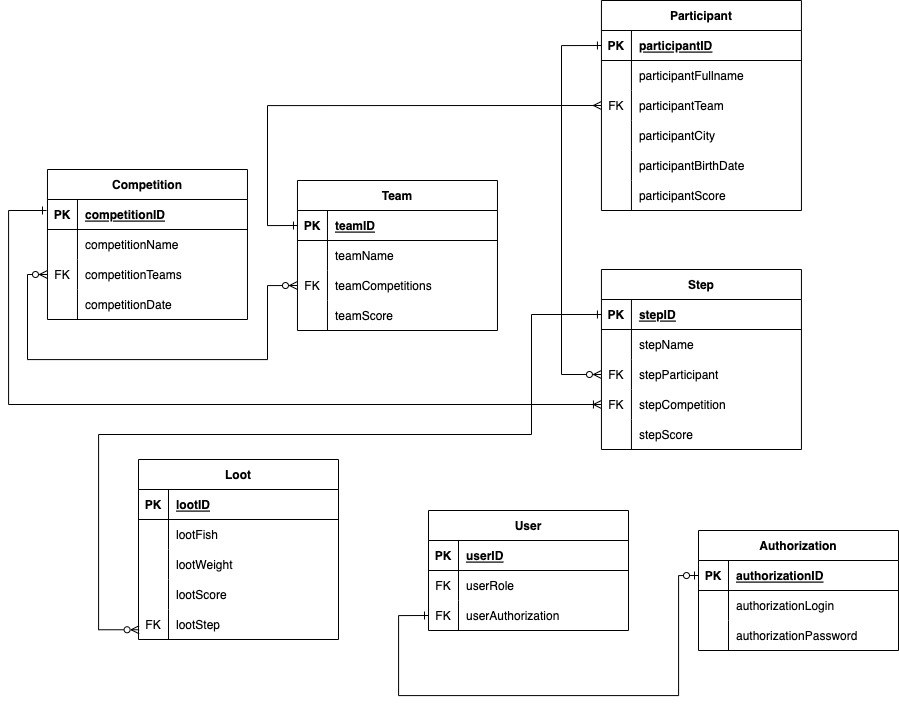
\includegraphics[scale=0.5]{img/er}}
	\caption{ER--диаграмма}
	\label{fig:er}
\end{figure}

\newpage


\subsection{Ролевая модель}

Ролевая модель предполагает наличие трех ролей: участника, судьи и администратора. Стоит отметить, что судья обладает всеми правами участника, а администратор --- всеми правами судьи.

Для успешной реализации поставленной задачи программа должна предоставлять следующие возможности:
\begin{itemize}[label=---]
	\item просмотр профилей участников;
	\item просмотр профилей команд;
	\item просмотр личного и командного рейтингов;
	\item просмотр личного и командного рейтингов по этапам;
	\item сортировка личного и командного рейтингов по убыванию/по возрастанию;
	\item сортировка личного и командного рейтингов по этапам по убыванию/по возрастанию.
\end{itemize}

Дополнительные возможности судьи:
\begin{itemize}[label=---]
	\item регистрация;
	\item авторизация;
	\item создание/редактирование/удаление соревнования;
	\item создание/редактирование/удаление команды;
	\item создание/редактирование/удаление участника;
	\item создание/редактирование/удаление зачета;
	\item создание/редактирование/удаление улова;
	\item внесение улова в зачет;
	\item добавление зачета в профиль участника;
	\item добавление участника в команду;
	\item добавление команды в соревнование;
	\item добавление зачета в соревнование.
\end{itemize}

Дополнительные возможности администратора:
\begin{itemize}[label=---]
	\item создание/редактирование/удаление профилей судей;
	\item создание/редактирование/удаление профилей администраторов;
\end{itemize}


\subsection{Проектирование приложения}

Приложение, разрабатываемое для iOS, может быть разделено на 3 части:
\begin{enumerate}
	\item слой бизнес логики --- взаимодействия между слоем доступа к данным и приложением: классы данных дублируют структуру базы данных;
	\item слой доступа к данным --- подключение к БД, отправка запросов, получение информации из БД;
	\item слой пользовательского интерфейса (UI) --- взаимодействие пользователя с программой.
\end{enumerate}

Сохранении последовательности представленных этапов поможет упростить разработку мобильного приложения.

\subsection{Вывод из раздела}

В данном разделе были спроектированы база данных и приложение, были формализованы требования к программе.
